\renewcommand{\nrandom}{\num{700}}
\renewcommand{\napplication}{\num{160}}
\newcommand{\ntoilet}{\num{77}}
\newcommand{\nmaxcount}{\num{26}}
\newcommand{\nsandcastle}{\num{25}}
\newcommand{\nconformant}{\num{24}}
\newcommand{\nmpec}{\num{8}}

\section{Evaluation}
\label{sect:erssat-evaluation}

We evaluated the proposed~\cref{alg:erssat} against
the state-of-the-art DPLL-based SSAT solver \dcssat~\cite{Majercik2005}
over both random $k$-CNF and application formulas.
The proposed algorithm is implemented in the \texttt{C++} language inside the \abc~\cite{ABC} environment.
The SAT solver \minisat-2.2~\cite{Een2003Solver} is used to answer satisfiability queries.
For weighted model counting,
we tried \cachet~\cite{Sang2004,Sang2005ModelCounting},
but the overall performance was not satisfactory.
Instead, we resorted to the well-developed BDD package \cudd~\cite{CUDD}.
Weight computation of a formula is fulfilled via a classic approach~\cite{Darwiche2002KnowledgeCompilation} that traverses the BDD of the formula and computes the satisfying probabilities of the BDD nodes.
Our prototyping implementation\footnote{Available at: \url{\ssatabcurl}} is named \erssat.
A bare version of \erssat without the enhancement techniques is called \erssatb in the experiments.
We used \ssatABCRevision in the experiments.

\subsection{Benchmark set}
The SSAT instances in the evaluation are hosted
in a publicly available database\footnote{Available at: \url{\ssatbenchmarkurl}}.
We used \ssatBenchRevision in the experiments.

\subsubsection{Random $k$-CNF formulas}
We generated random $k$-CNF formulas by \cnfgen~\cite{Lauria2017CNFgen}.
A collection of~\nrandom~formulas were generated with $k$,
i.e., the number of literals in a clause,
taking values from $\{3,4,5,6,7,8,9\}$,
the number of variables taking values from $\{10,20,30,40,50\}$,
and clause-to-variable ratio taking values from $\{k-1,k,k+1,k+2\}$.
Five formulas were sampled for each parameter combination.
To convert the propositional formulas into E-MAJSAT formulas,
the first half of the variables are existentially quantified,
and the rest are randomly quantified with probability $0.37$.

\subsubsection{Application formulas}
\begin{table}[ht]
    \centering
    \caption{The families of the application formulas}
    \label{tbl:exist-random-ssat-families}
    \begin{tabular}{c|c|c}
        Family               & Description                                            & Number       \\
        \hline
        \textit{Toilet-A}    & Adapted from exist-forall QBFs~\cite{Narizzano2006}    & \ntoilet     \\
        \textit{Conformant}  & Adapted from exist-forall QBFs~\cite{Narizzano2006}    & \nconformant \\
        \textit{Sand-Castle} & A probabilistic planning problem~\cite{Majercik1998}   & \nsandcastle \\
        \textit{Max-Count}   & Adapted from maximum model counting~\cite{Fremont2017} & \nmaxcount   \\
        \textit{MPEC}        & Probabilistic design equivalence checking              & \nmpec       \\
    \end{tabular}
\end{table}

We collected five families of application formulas for evaluation.
Their descriptions and the numbers of the instances in each family are summarized in~\cref{tbl:exist-random-ssat-families}.
The first two families,
\textit{Toilet-A} and \textit{Conformant},
were adapted from exist-forall-exist QBFs~\cite{Narizzano2006}.
We converted the QBFs into exist-random-exist quantified SSAT formulas
by replacing their universal quantifiers with randomized ones with probabilities $0.5$.
The third family \textit{Sand-Castle} is a probabilistic conformant planning domain.
The problem can be encoded as E-MAJSAT formulas~\cite{Majercik1998}.
The family \textit{Max-Count} models the problems of maximum satisfiability, quantitative information flow, and program synthesis with maximum model counting~\cite{Fremont2017}.
We represented the maximum model counting instances as E-MAJSAT formulas.
The last family \textit{MPEC} consists of formulas that analyze the maximum probability of a probabilistic circuit to produce erroneous outputs.
%The MPEC formulas for evaluation were created from \texttt{ISCAS} benchmark suite with the erroneous and defective rates equal to $0.125$ and $0.01$.

\subsection{Experimental setup}
Our experiments were performed on a machine with
one 2.2\,GHz CPU (Intel Xeon Silver 4210) with 40~processing units and 134616\,MB of RAM.
The operating system was Ubuntu~20.04 (64~bit),
using Linux~5.4.
The programs were compiled with \texttt{g++ 9.3.0}.
Each SSAT-solving task was limited to a CPU core,
a CPU time of \SI{15}{min},
and a memory usage of \SI{8}{GB}.
To achieve reliable benchmarking,
we used a benchmarking framework \benchexec\footnote{Available at: \url{\benchexecurl}}~\cite{Benchmarking-STTT}.
%%% TODO: fix the evaluation commit
%and \experimentRevision of \cpachecker for evaluation.

\subsection{Results}

\subsubsection{Random $k$-CNF formulas}

\begin{figure*}[ht]
    \centering
    \subfloat[CPU time]{
        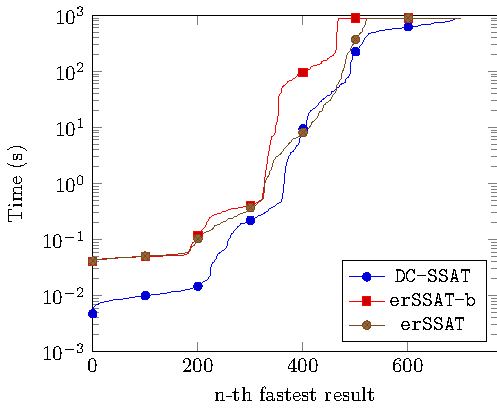
\includegraphics{exist-random-ssat/evaluation/plots/quantile-cputime-Random.pdf}
        \label{fig:erssat-quantile-cputime-random}
    }\\
    \subfloat[Memory usage]{
        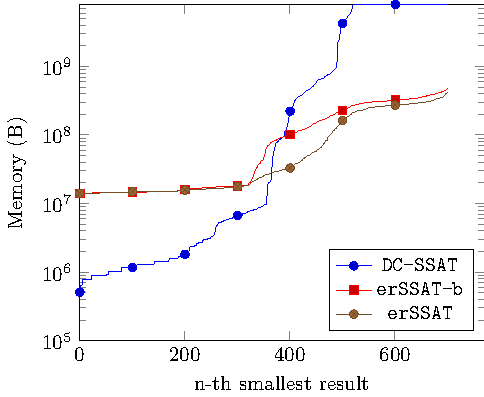
\includegraphics{exist-random-ssat/evaluation/plots/quantile-memory-Random.pdf}
        \label{fig:erssat-quantile-memory-random}
    }
    \caption{Quantile plots of random $k$-CNF formulas}
    \label{fig:erssat-quantile-random}
\end{figure*}

\Cref{fig:erssat-quantile-random} shows the quantile plots regarding CPU time and memory usage
of the SSAT instances derived from the random $k$-CNF formulas.
A data point $(x,y)$ in a quantile plot indicates that
there are $x$ formulas processed by the respective algorithm within a resource constraint of $y$.
In~\cref{fig:erssat-quantile-cputime-random},
we observe that \erssat solved a similar amount of formulas as \dcssat did.
Moreover, the enhancement techniques improve the performance of \erssat a lot,
as can be seen from the huge difference between \erssat and \erssatb.
On the other hand,
\cref{fig:erssat-quantile-memory-random} shows that the memory usage of \dcssat is much larger than that of \erssat.
This can be attributed to the subformula caching of \dcssat.
Instead, \erssat only builds BDDs for cofactored formulas, which confined its memory footprint.

\subsubsection{Application formulas}

\begin{figure*}[ht]
    \centering
    \subfloat[CPU time]{
        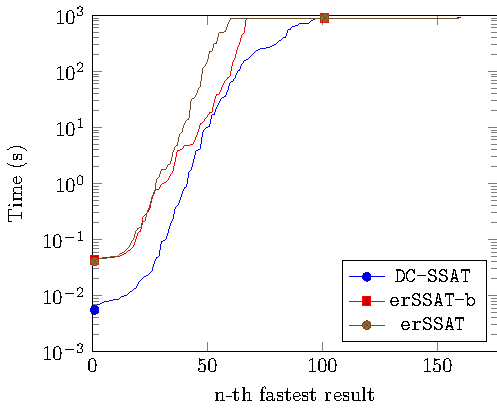
\includegraphics{exist-random-ssat/evaluation/plots/quantile-cputime-Application.pdf}
        \label{fig:erssat-quantile-cputime-application}
    }\\
    \subfloat[Memory usage]{
        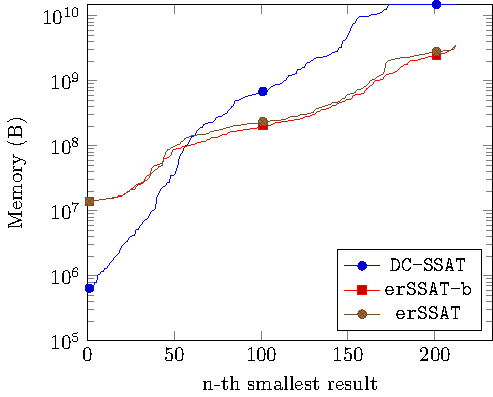
\includegraphics{exist-random-ssat/evaluation/plots/quantile-memory-Application.pdf}
        \label{fig:erssat-quantile-memory-application}
    }
    \caption{Quantile plots of application formulas}
    \label{fig:erssat-quantile-application}
\end{figure*}

\begin{figure*}[ht]
    \centering
    \subfloat[\erssatb]{
        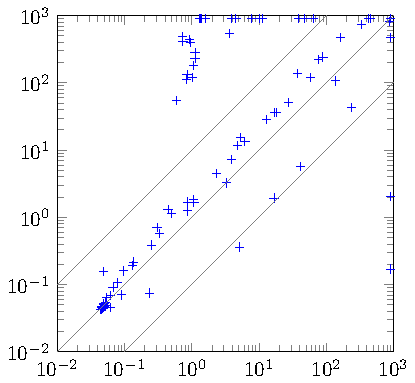
\includegraphics{exist-random-ssat/evaluation/plots/scatter-erssat.pdf}
        \label{fig:erssat-scatter-cputime-application}
    }\\
    \subfloat[\dcssat]{
        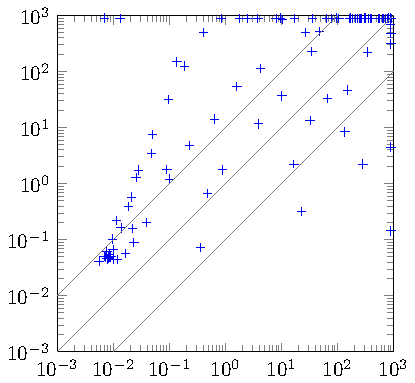
\includegraphics{exist-random-ssat/evaluation/plots/scatter-dcssat.pdf}
        \label{fig:dcssat-scatter-cputime-application}
    }
    \caption{CPU-time scatter plots of application formulas with \erssat in y-axis and compared approaches in x-axis}
    \label{fig:erssat-scatter-application}
\end{figure*}

% Commands for application formulas of ER-SSAT
\newcommand{\dcssatToiletA}{\num{44}}
\newcommand{\dcssatconformant}{\num{1}}
\newcommand{\dcssatcastle}{\num{21}}
\newcommand{\dcssatMaxCount}{\num{2}}
\newcommand{\dcssatMPEC}{\num{3}}
\newcommand{\erssatbToiletA}{\num{45}}
\newcommand{\erssatbconformant}{\num{1}}
\newcommand{\erssatbcastle}{\num{14}}
\newcommand{\erssatbMaxCount}{\num{1}}
\newcommand{\erssatbMPEC}{\num{1}}
\newcommand{\erssatToiletA}{\num{38}}
\newcommand{\erssatconformant}{\num{2}}
\newcommand{\erssatcastle}{\num{13}}
\newcommand{\erssatMaxCount}{\num{3}}
\newcommand{\erssatMPEC}{\num{2}}

\begin{table}[ht]
    \centering
    \caption{The number of solved instances per family}
    \label{tbl:solved-instances-per-family}
    \begin{tabular}{c|c|c|c}
        Family               & \dcssat           & \erssatb           & erssat            \\
        \hline
        \textit{Toilet-A}    & \dcssatToiletA    & \erssatbToiletA    & \erssatToiletA    \\
        \textit{Conformant}  & \dcssatconformant & \erssatbconformant & \erssatconformant \\
        \textit{Sand-Castle} & \dcssatcastle     & \erssatbcastle     & \erssatcastle     \\
        \textit{Max-Count}   & \dcssatMaxCount   & \erssatbMaxCount   & \erssatMaxCount   \\
        \textit{MPEC}        & \dcssatMPEC       & \erssatbMPEC       & \erssatMPEC       \\
    \end{tabular}
\end{table}

\Cref{fig:erssat-quantile-application} shows the quantile plots of the application SSAT formulas.
To our surprise, the results are very different from those of random $k$-CNF formulas.
First, \dcssat solved the most instances.
Second, the bare version \erssatb solved more instances than \erssat did.
In order to investigate this phenomenon,
the scatter plots are shown in~\cref{fig:erssat-scatter-application}.
A data point $(x,y)$ in the plots indicates that there is a formula processed by both \erssat and a compared approach,
while \erssat took a CPU time of $y$~seconds and the other approach took a CPU time of $x$~seconds.
The numbers of instanced solved per family are summarized in~\cref{tbl:solved-instances-per-family}.